%% ----------------------------------------------------------------
%% Introduction.tex
%% ---------------------------------------------------------------- 
\chapter{Introduction} \label{Chapter:Introduction}
You probably found all the files from \cite{Longman:2019:templ},
they were originally made from \cite{Gunn:2001:pdflatex}.
Template specific instructions can be found at:
\url{https://git.soton.ac.uk/el7g15/uos-latex-template-instructions}.

\tref{Table:tabex} illustrates the results of some arbitrary example work.
\begin{table}[!htb]
  \centering
  \begin{tabular}{cc}
  \toprule
  \textbf{Training Error} & \textbf{Testing Error}\\
  \midrule
  0 & $\infty$\\
  \bottomrule
  \end{tabular}
  \caption{The Results}
  \label{Table:tabex}
\end{table}

\fref{Figure:figex} shows why this is the case.
\begin{figure}[!htb]
  \centering
  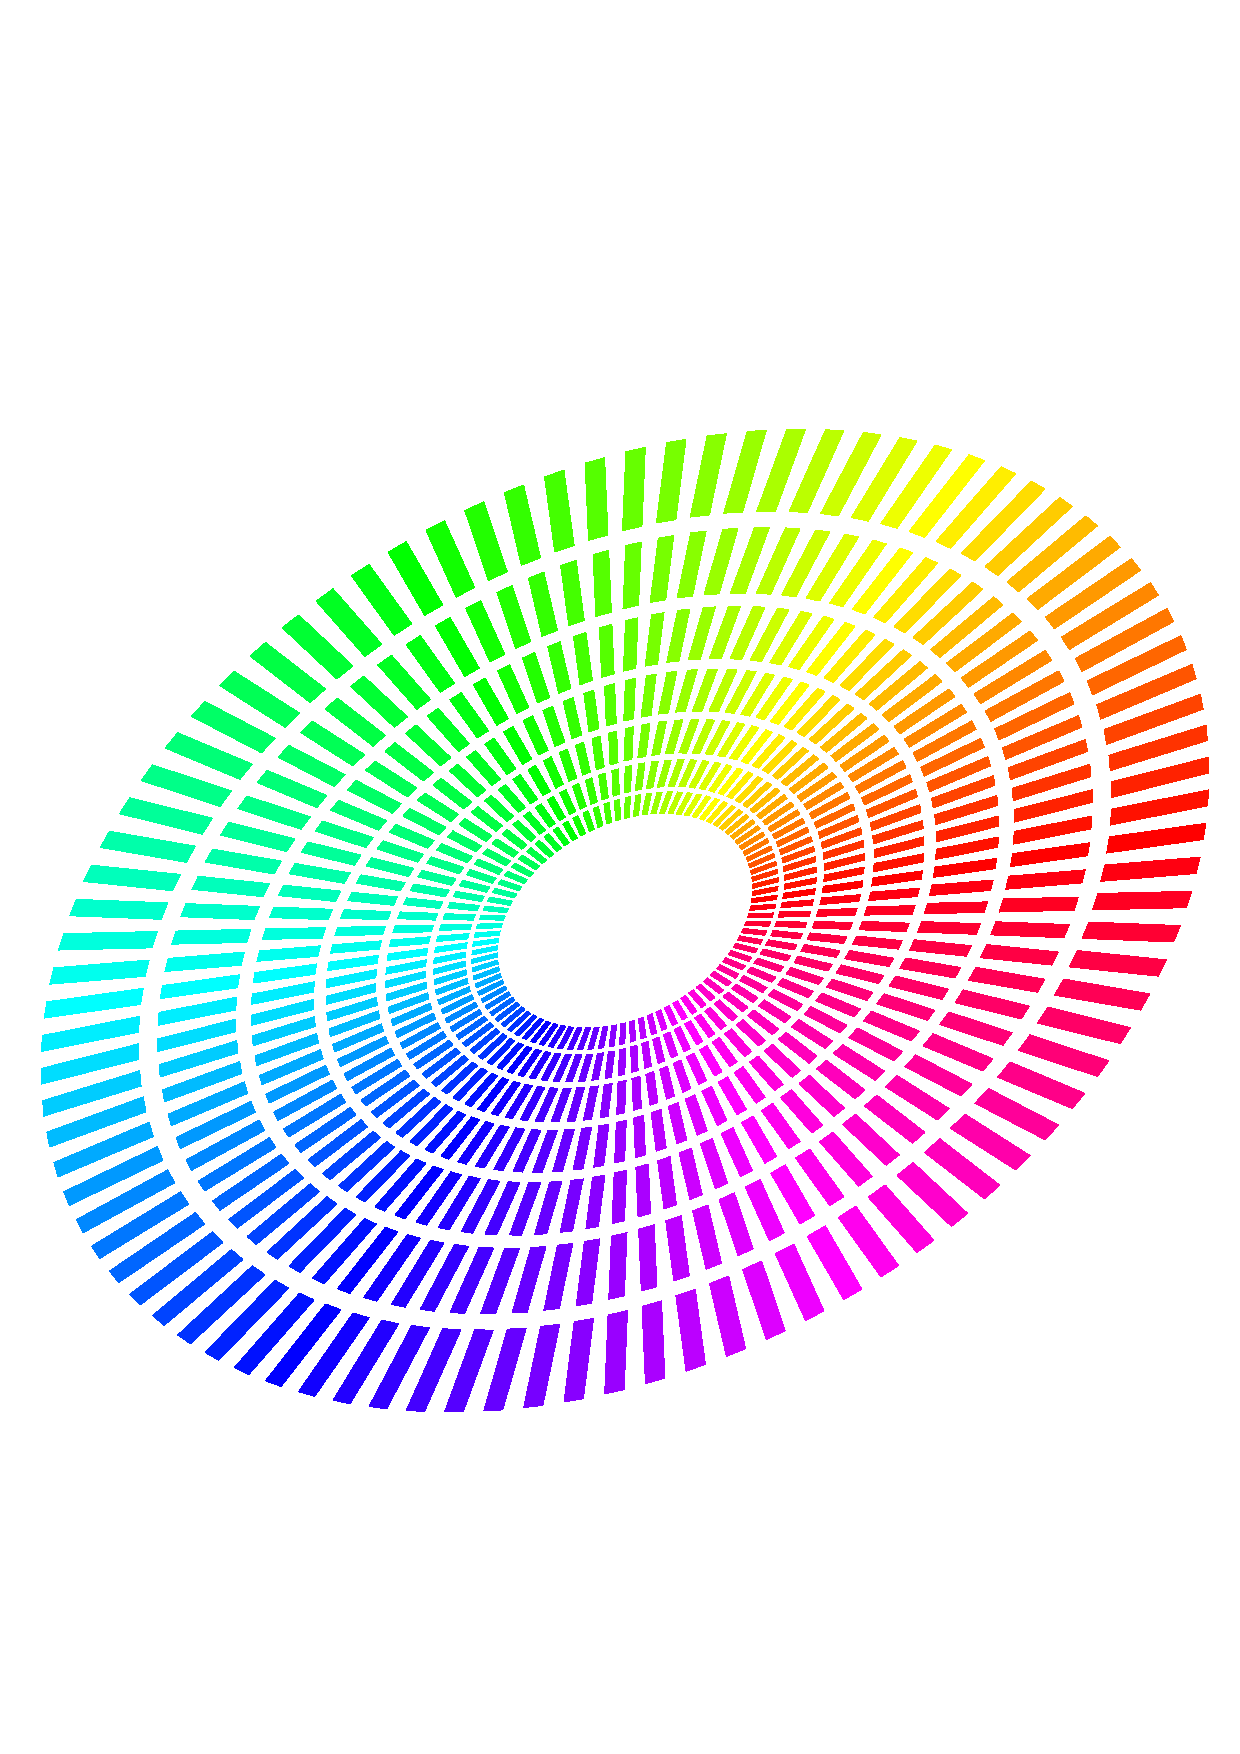
\includegraphics[width=8cm]{figure}
  \caption{A colourful picture.}
  \label{Figure:figex}
\end{figure}

This page shows you a subfigure example in \fref{Figure:figsubex}.
\begin{figure}[!htb]
  \centering
  \subcaptionbox{The left caption}{
    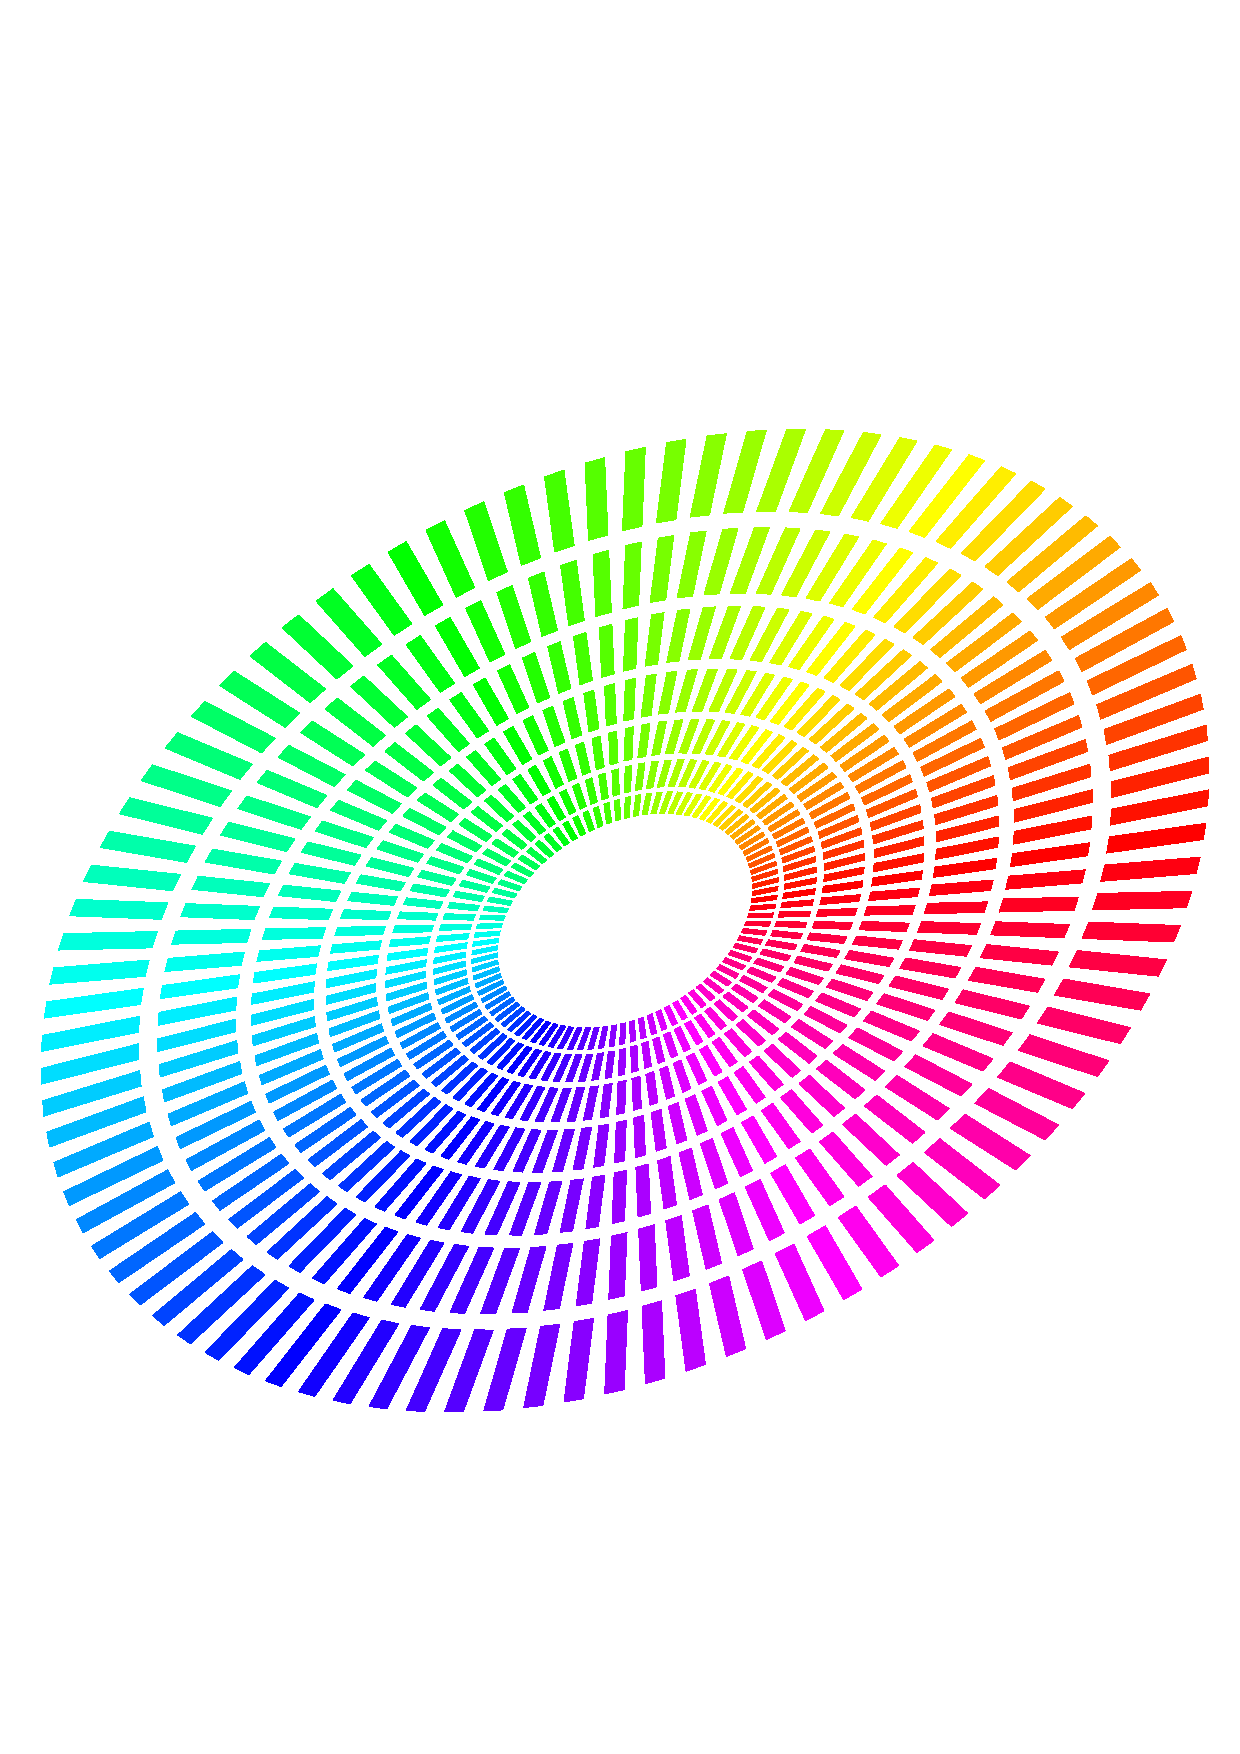
\includegraphics[width=4.2cm]{figure}
    \label{Figure:figsubex:left}
  }
  \subcaptionbox{The right caption}{
    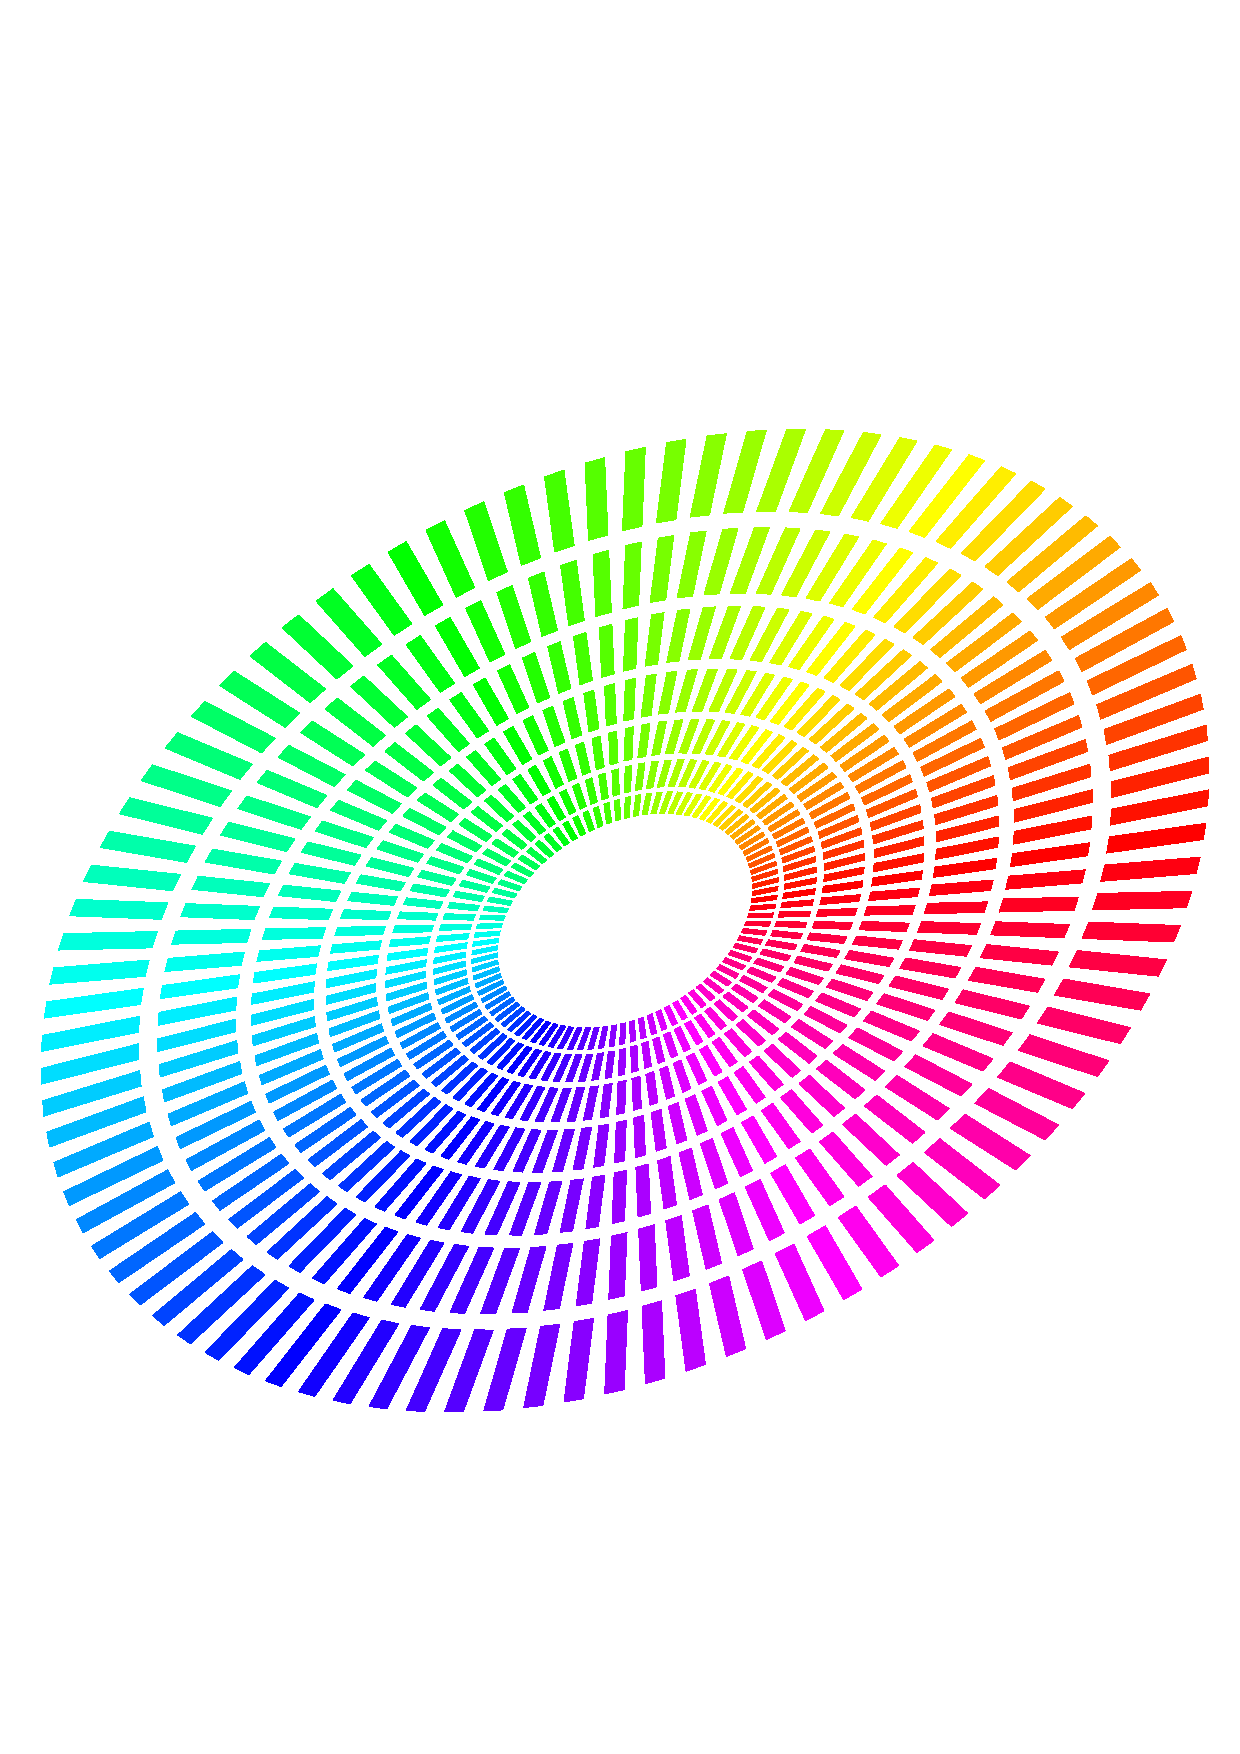
\includegraphics[width=4.2cm]{figure}
    \label{Figure:figsubex:right}
  }
  \caption{A doubly colourful picture.}
  \label{Figure:figsubex}
\end{figure}
Lorem ipsum dolor sit amet, consectetur adipiscing elit. Donec rutrum sodales ligula, ac aliquam sem interdum at. Ut commodo pulvinar ipsum. Aliquam et diam sed nibh tincidunt mollis vitae quis nunc. In vel ante vitae felis semper malesuada sed a metus. Aliquam semper metus vel metus imperdiet, quis mollis nisi volutpat. Integer in convallis erat, et auctor dui. Phasellus id tristique tortor. Mauris ac nisi ut mi pulvinar interdum. Donec quis nibh tempus erat lobortis dapibus non a nunc. Nulla laoreet tempus fringilla. Aliquam pulvinar, sapien eu interdum gravida, libero urna dapibus sem, sodales efficitur lorem nunc et justo. Proin vitae dolor nisl.

\section{A Section of a chapter}
Nulla molestie velit sed dui ullamcorper viverra. Fusce placerat vulputate lacus eu consequat. Cras ullamcorper vel mauris quis aliquam. Curabitur non varius elit, eget commodo urna. Phasellus erat libero, faucibus elementum augue eget, malesuada fringilla purus. Quisque pulvinar, lectus sit amet ultricies tristique, eros nunc commodo lacus, nec ultrices risus lorem vitae diam. Cras ac ornare nisi.

\subsection{Some quotes}

Nam egestas felis euismod erat tincidunt ornare. Nulla hendrerit tempor purus ac consequat. Aliquam commodo, ipsum vestibulum lobortis semper, urna turpis sagittis dolor, id ullamcorper nulla nisl vitae ex. Vivamus ut metus vel velit rhoncus pulvinar sit amet nec diam. Aliquam aliquet, enim eget efficitur euismod, velit arcu mattis nisl, a mollis dui leo vel libero. Nullam porttitor convallis magna ut feugiat. `Cras at ultrices metus.' Nullam vulputate quis justo sit amet pharetra. Praesent sodales eros non suscipit gravida.
\begin{quote}
Lorem ipsum dolor sit amet, consectetur adipiscing elit. Donec rutrum sodales ligula, ac aliquam sem interdum at.
\end{quote}

Pellentesque sodales lobortis feugiat. Vivamus volutpat mauris id odio aliquam maximus sed sit amet nibh. Fusce odio tortor, aliquam et mauris facilisis, interdum placerat tortor. Suspendisse dapibus, massa eget cursus congue, mi lectus luctus nisl, vitae sagittis ligula ante sit amet enim. Donec quis sapien vel ex vestibulum porta. Vivamus mattis sodales turpis, id interdum justo ullamcorper a. Aenean ornare urna turpis, id fermentum eros commodo aliquet. Class aptent taciti sociosqu ad litora torquent per conubia nostra, per inceptos himenaeos. Donec cursus pretium ex at mollis. Vestibulum ante ipsum primis in faucibus orci luctus et ultrices posuere cubilia Curae; Sed at diam quam. Etiam a sollicitudin dui. Nulla facilisi. Phasellus condimentum tincidunt ipsum. Sed dignissim neque a porttitor finibus. Maecenas pretium dictum lorem vitae viverra.
\begin{quote}
The \verb|\attrib| macro attributes block elements, for example when citing
a reference after a block quotation.
\ifdefined\attrib\attrib{\cite{attribpackage}}\fi
\end{quote}

Donec vitae massa nisi. Praesent sed sollicitudin urna. Suspendisse vitae cursus tortor. In egestas quis dolor ac porttitor. Pellentesque suscipit leo nisi, a semper nunc interdum quis. Aenean massa magna, aliquam imperdiet lorem vitae, vestibulum dignissim nunc. Nunc molestie eleifend dui et porta. Sed auctor eu nunc vel faucibus. Integer et finibus metus, pharetra egestas velit. Sed nec magna semper, rutrum diam vitae, accumsan sapien. Donec congue viverra luctus.
